\begin{figure}[t]
    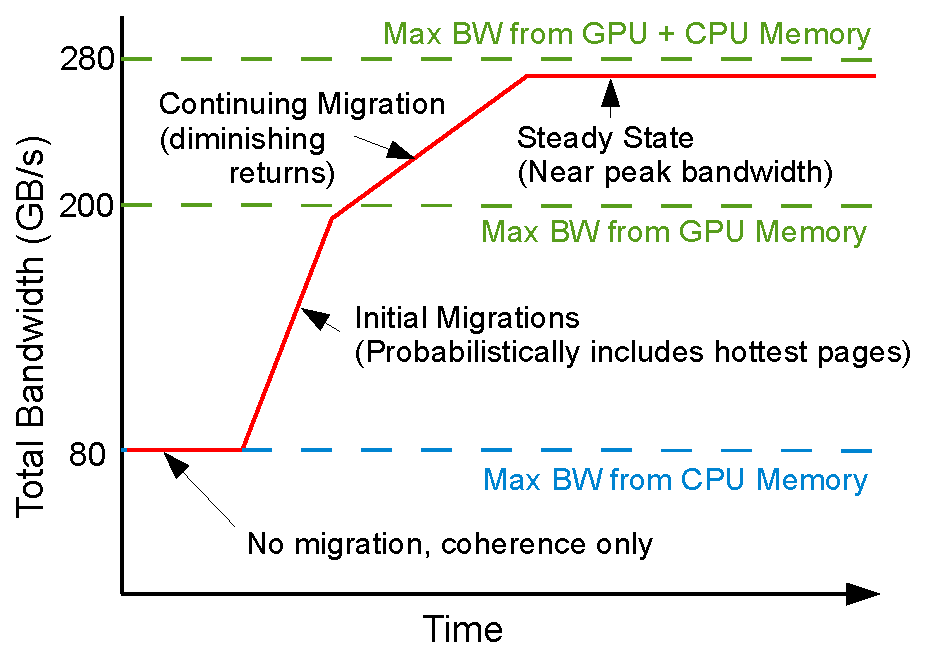
\includegraphics[width=\columnwidth]{hpca2015/figures/opportunity.eps} 
    \caption{Opportunity cost of relying on cache coherence versus migrating pages near beginning of application run.}
    \label{fig:opportunity}
\end{figure}

\vspace{-0.05in}
\section{Balancing Page Migration and Cache-Coherent Access}
\label{threshold}

In the future, it is likely GPUs and CPUs will use a shared page table structure
while maintaining local TLB caches.  It remains to be seen if the GPU will be
able to natively walk the operating system page tables to translate virtual to
physical address information, or if GPUs will use an IOMMU-like hardware in
front of the GPU's native TLB to perform such translations.  In either case, the
translation from virtual to physical addresses will be implicit, just as it is
today for CPUs, and will no longer require trapping back to the CPU to translate
or modify addresses.  As a result, when page mappings must be modified, all
CPUs---and now the GPU---must follow appropriate steps to safely invalidate
their local TLB caches.  While CPUs typically use a TLB per CPU-core, GPUs use a
multi-level global page table across all compute pipelines.  Therefore, when TLB
shootdowns occur, the penalty will not stall just a single CPU pipeline, it is
likely to stall the entire GPU\@. Whereas recent research has proposed intra-GPU
sharer tracking~\cite{Villavieja2011} that could mitigate these stalls, this
additional hardware is costly and typically unneeded for graphics applications
and thus may not be adopted in practice.

Figure~\ref{fig:opportunity} provides a visual representation of the effect of
balancing memory accesses from both DDR (CPU-attached) and GDDR (GPU-attached)
memory. Initially, pages reside entirely in DDR memory.  Without migration, the
maximum bandwidth available to GPU accesses (via cache coherence to the DDR
memory)  will be limited by either the interconnect or DDR memory bandwidth.  As
pages are migrated from DDR to GDDR, the total bandwidth available to the GPU
rises as pages can now be accessed concurrently from both memories.  Migrations
that occur early in kernel execution will have the largest effect on improving
total bandwidth, while later migrations (after a substantial fraction of GDDR
memory bandwidth is already in use) have less effect.  Performance is maximized
when accesses are split across both channels in proportion to their peak
bandwidth.  Figure~\ref{fig:opportunity} shows the total bandwidth that is
wasted if pages are not migrated eagerly, early in kernel execution.  The key
objective of the migration mechanism is to migrate the hottest pages as early as
possible to quickly ramp up use of GDDR memory bandwidth.  Nevertheless,
migrating pages that are subsequently never accessed wastes bandwidth on both
memory interfaces.  In this section, we investigate alternative DDR-to-GDDR
memory migration strategies.  In particular, we contrast a simple, eager
migration strategy against more selective strategies that try to target only hot
pages.

\subsection{Methodology}
To evaluate page migration strategies, we model a GPU with a heterogeneous
memory system comprising both  GDDR and DDR memories. We discuss our baseline
simulation framework in Chpater~\ref{chap:methodology}.
%The GDDR memory is directly attached and addressable by the GPU, as in existing
%systems.  We assume DDR memory may be accessed by the GPU via a
%cache-line-granularity coherent interface at an additional 100 GPU cycle
%latency (in addition to the DDR access latency).  We derive our latency
%estimates from SMP CPU interconnects~\cite{INTELXEON}.  We find that these
%additional 100 cycles of latency have relatively little impact on GPU
%application performance (compared to a hypothetical baseline with no additional
%latency), as GPUs are already effective in hiding such latency.  Across the
%suite of applications we study, the mean performance degradation due to
%interconnect latency is 3\%, and at worst 10\%.
%
%We extend GPGPU-Sim~\cite{gpgpusim_ispass09} with a model of this GDDR5-DDR4
%heterogeneous memory.
Table~\ref{tab:mig-methodology} lists memory configuration of our simulation
framework.
%We make several additional enhancements to the baseline GTX-480 model to better
%match the bandwidth requirements of future GPUs (e.g., increasing the number of
%miss status handling registers, increasing clock frequency, etc).  We assume a
%GDDR bandwidth of 200GB/s and a DDR bandwidth of 80 GB/s.

\begin{table}[t]
\begin{center}
\begin{tabular}{|l|l|}
%\hline
%Simulator & GPGPU-Sim 3.x\\
%\hline
%GPU Arch & NVIDIA GTX-480 Fermi-like\\
%\hline
%GPU Cores& 15 {\color{black}SMs} @ 1.4Ghz\\
%\hline
%L1 Caches & 16kB/SM \\
%\hline
%L2 Caches & Memory Side 128kB/DRAM Channel\\
%\hline
%L2 MSHRs & 128 Entries/L2 Slice\\
%\hline
\hline
\multicolumn{2}{|c|}{Memory system}\\
\hline
GPU-Local GDDR5 & 8-channels, 200GB/sec aggregate\\
\hline
GPU-Remote DDR4& 4-channels, 80GB/sec aggregate\\
\hline
DRAM Timings & \multicolumn{1}{|l|}{RCD=RP=12,RC=40,CL=WR=12}\\
\hline
GPU-CPU &  100 GPU core cycles\\
Interconnect Latency & \\
\hline
\end{tabular}
\caption{Memory system configuration for heterogenous CPU-GPU system.}
\label{tab:mig-methodology}
\end{center}
\end{table}

We model a software page migration mechanism in which migrations are performed
by the CPU based on hints provided asynchronously by the GPU\@.  The GPU tracks
candidate migration addresses by maintaining a ring buffer of virtual addresses
that miss in the GPU TLB.  The runtime process on the CPU polls this ring
buffer, converts the address to the page aligned base address and initiates
migration using the standard Linux {\tt move\_pages} system call.

As in a CPU, the GPU TLB must be updated to reflect the virtual address changes
that result from migrations.  We assume a conventional x86-like TLB shootdown
model where the entire GPU is treated like a single CPU using traditional
interprocessor interrupt shootdown.  In future systems, an IOMMU performing
address translations on behalf of the GPU cores is likely to hide the specific
implementation details of how it chooses to track which GPU pipelines must be
stalled and flushed during any given TLB shootdown.  For this work, we make a
pessimistic assumption that, upon shootdown, all execution pipelines on the GPU
must be flushed before the IOMMU handling the shootdown on behalf of the GPU can
acknowledge the operation as complete. We model the time required to invalidate
and refill the TLB entry on the GPU as a parameterized, fixed number, of cycles
per page migration. In Section~\ref{thresholdresults} we examine the effect of
this invalidate/refill overhead on the performance of our migration policy,
recognizing that the implementation of TLB structures for GPUs is an active area
of research~\cite{Pichai2014,Power2014}.

We model the memory traffic due to page migrations without any special
prioritization within the memory controller and rely on the software runtime to
rate-limit our migration bandwidth by issuing no more than 4 concurrent page
migrations.  We study our proposed designs using memory intensive workloads from
Rodinia~\cite{Che2009} and some other recent HPC
applications~\cite{comd,cns,minife,xsbench}. These benchmarks cover varied
application domains, including graph-traversal, data-mining, kinematics, image
processing, unstructured grid, fluid dynamics and Monte-Carlo transport
mechanisms.
